\chapter{Concetti base del Cloud Computing}
Consideriamo il normale utilizzo di un computer. Avendo a disposizione una capacità di calcolo fissata, può capitare lo scenario illustrato di seguente:

\begin{figure}[ht]
    \centering
    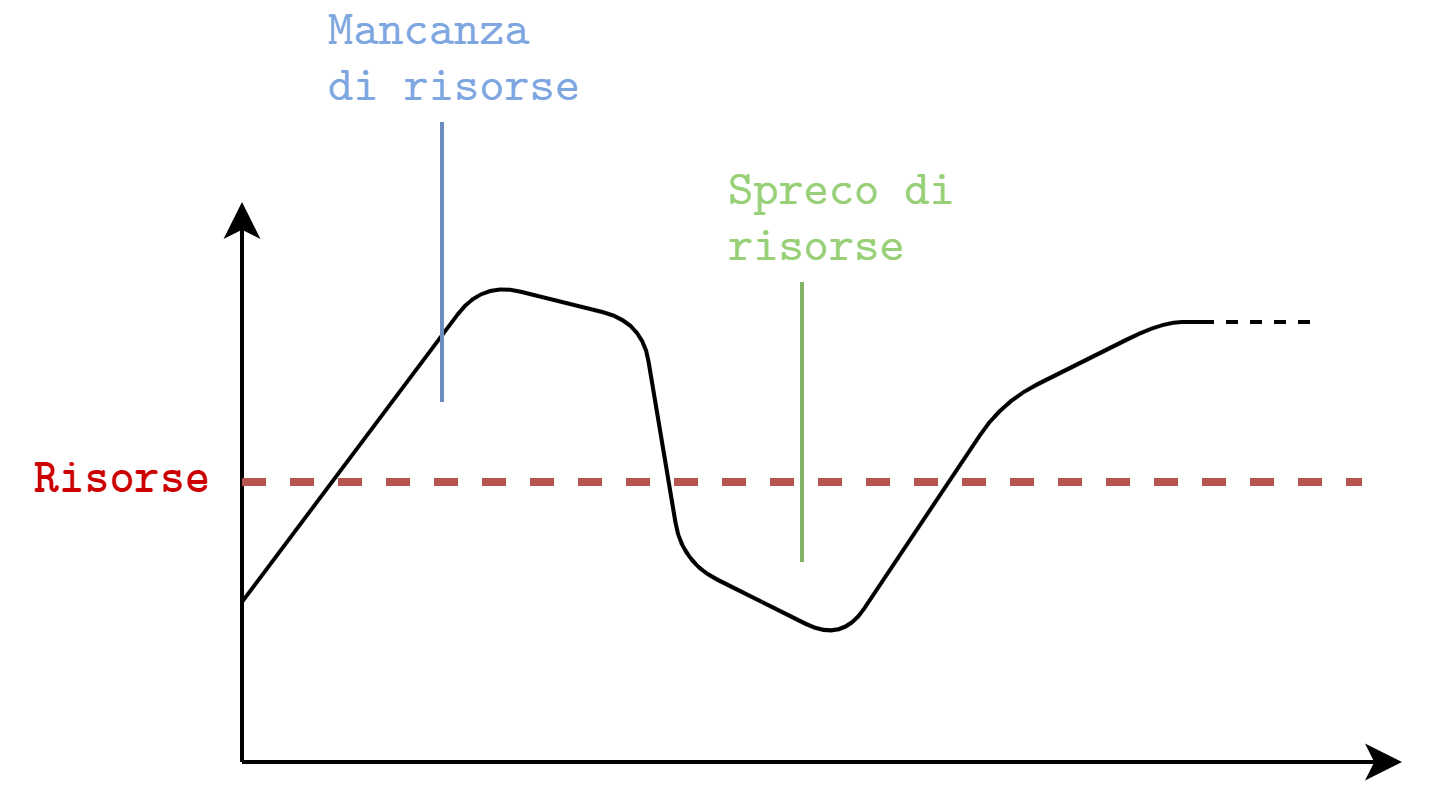
\includegraphics[width=8cm]{./Images/cap2/2.1.png}
    \label{fig:image2.1}
\end{figure}

In media vengono utilizzati il 10\% di CPU, il 60\% di memoria e il 20\% di larghezza di banda.

\section{Le origini}
Le prime tracce di quello che si può definire \textbf{Cloud computing} risalgono al 1961, quando lo scienziato John McCarthy affermò che in breve tempo sarebbe stato possibile usufruire della capacità di calcolo come una risorsa pubblica.

Verso fine anni '90 Salesforce.com iniziò a fornire servizi di gestione dell'azienda. Solo nel 2002 Amazon fece debuttare il primo servizio di Cloud computing, \textbf{Amazon Elastic Compute Cloud} (EC2).

\section{Definizioni}
Nel corso degli anni sono state presentate diverse definizioni di \textbf{Cloud computing}, tutte legate all'utilizzo che se ne faceva nel periodo di riferimento. 

La prima definizione fu data dalla multinazionale Gartner:

\begin{displayquote}
\textit{"...a style of computing in which scalable and elastic IT-enabled capabilities are delivered as a service to external customers using Internet technologies."}
\end{displayquote}


Il concetto espresso da questa definizione si rifà a scalabilità ed elasticità. Il cloud computing in questo senso è uno stile di calcolo che cambia le modalità con cui siamo stati abituati a fare computazioni.
Successivamente fu la Forrester Research che provò a dare una definizione:
\begin{displayquote}
\textit{"...a standardized IT capability (service, software or infrastructure) delivered via Internet technologies in a pay-per-use, self-service way."}
\end{displayquote}
Qui vengono introdotti gli importanti concetti di \textbf{pay-per-use} e \textbf{self-service}, che offrono vantaggi come indipendenza dalla piattaforma e flessibilità, ma anche degli svantaggi come la complessità, in quanto esistono migliaia di servizi, e sapersi orientare richiede tempo. Possiamo dire che c'è una sorta di barriera di ingresso.

\vspace{5mm}

La definizione data dal NIST invece risale al 2011:
\begin{displayquote}
\textit{"Cloud computing is a model for enabling ubiquitous, convenient, on-demand network access to a shared pool of configurable computing resources that can be rapidly provisioned and released with minimal management effirt or service provider interaction. This cloud model is composed of five essential characteristics, three service models, and four deployment models."}
\end{displayquote}
In pratica questa definizione afferma che il Cloud computing è un modello di calcolo per abilitare accesso alla rete on-demand su una serie di risorse di calcolo configurabili. Questo garantisce una fornitura veloce, quindi poca interazione con il provider. Inoltre per la prima volta si parla di \textit{modello di calcolo}: questo rappresenta un passo avanti rispetto al modello di calcolo precedente.

Infine, la definizione del libro di testo adottato:
\begin{displayquote}
\textit{"Cloud computing is a specialized form of distribuited computing that introduces utilization models for remotely provisioning scalable and measured resources."}
\end{displayquote}

Ovvero si parla di una forma di calcolo distribuito che fornisce risorse scalabili accessibili da remoto e misurate. Quindi possiamo affermare che il cloud computing è una diretta evoluzione del calcolo distribuito. È importante enfatizzare anche il concetto di risorse misurate, in quanto la gestione dei costi è uno degli argomenti principali su cui approfondire.

\section{Business Drivers}
Alcune delle nozioni fondamentali definite in questo capitolo si basano sullo scenario principale, che vede opporsi i \textbf{cloud provider}, che offrono infrastrutture e servizi, e i \textbf{cloud consumer}, rappresentati dagli utilizzatori delle infrastrutture sia in modo privato che in modo aziendale.

Il mercato generato dal cloud quindi è influenzato da entrambi i lati, ed è questo che spinge le organizzazioni a diventare cloud provider.
Possiamo distinguere tre business driver:
\begin{itemize}
    \item capacity planning;
    \item cost reduction;
    \item operational agility.
\end{itemize}

\break
\subsection{Capacity planning}
Il \textbf{capacity planning} è il processo utilizzato per prevedere i servizi e le richieste future da utilizzare partendo dai dati a disposizione. \textit{Avrò bisogno di un nuovo disco tra un anno? Il servizio che sto utilizzando ora è sufficiente?}

La capacity è la massima capacità di lavoro che una risorsa può fornire nel tempo, e deve infacciarsi con la richiesta. Una discrepanza tra la capacità di una risorsa IT e la domanda di questa risorsa può rendere tutto il sistema inefficiente. La previsione della quantità di risorse da utilizzare deve essere il più precisa possibile, in quanto può portare ad un \textit{overprovisioning} o a un \textit{underprovisioning}.
Il primo scenario si verifica nel caso non viene utilizzata la totalità della capacity che è stata pagata, mentre il secondo è nel caso opposto, ovvero quando non sono state allocate abbastanza risorse.


\begin{figure}[ht]
    \centering
    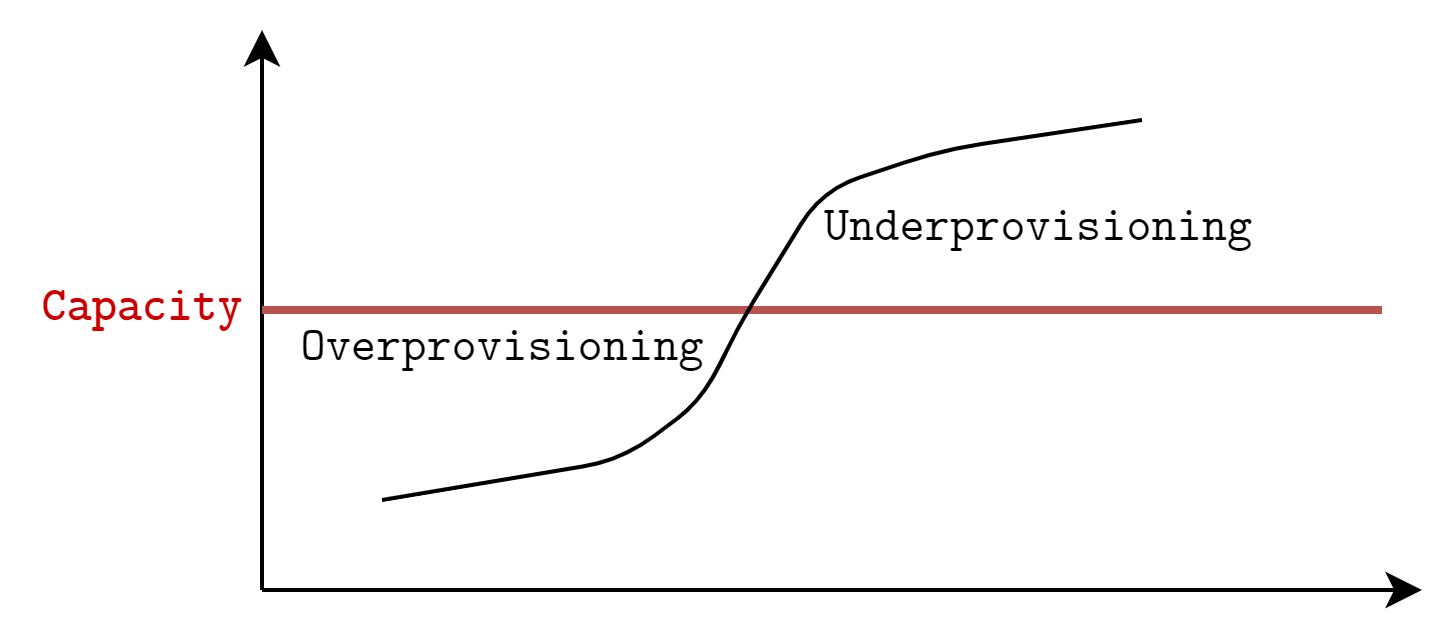
\includegraphics[width=8cm]{./Images/cap2/2.2.png}
    \label{fig:image2.2}
\end{figure}


Al contrario di come può sembrare, sono entrambi scenari negativi, in quanto non ci dimentichiamo che stiamo pagando la capacity. Per questo si parla di \textit{planning} per minimizzare la discrepanza.
Possiamo distinguere tre diverse strategie di capacity planning:
\begin{itemize}
    \item \textbf{Lead strategy}: aggiungere capacità a una risorsa IT in anticipo rispetto alla domanda;
    \item \textbf{Lag strategy}: aggiungere capacità quando questa raggiunge la sua capacità massima;
    \item \textbf{Match strategy}: aggiungere capacità in piccoli incrementi, insieme all'aumento della domanda.
\end{itemize}
Il capacity planning può essere difficile in quanto c'è bisogno spesso di investimenti e soprattutto non è semplice prevedere le necessità esatte di una certa risorsa.

\subsection{Cost Reduction}
Il business generato dal cloud ha delle prestazioni che vanno tutelate, per cui ci sono dei costi da affrontare. Possiamo distinguere due tipi di spese:
\begin{itemize}
    \item le spese in conto capitale ovvero spese immobilizzate, come l'acquisto di beni immobiliari e di infrastrutture (server, rack, postazioni per il raffreddamento o gruppi di continuità). 
    \item le spese operative sono rappresentate dai costi correnti: una volta acquistata l'infrastruttura c'è bisogno di pagare un system manager per configurarla, degli assistenti, un'azienda di pulizia per i locali, senza dimenticare le spese per mantenere l'infrastruttura (stipendi, fitti, manutenzione).
\end{itemize}
\begin{mdframed}[backgroundcolor=gray!40,shadow=false]
\textbf{Le spese in conto capitale generano sempre spese operative.} 

Questo perchè oltre al fatto che i costi operativi superano quelli in conto capitale, bisogna attuare misure di sicurezza per proteggere le proprie infrastrutture, e non parliamo di cybersecurity ma proprio di sicurezza fisica! Quindi ci saranno spese come opportune serrature, guardie notturne, ecc. A queste poi si aggiungono le spese amministrative per il supporto e le licenze. Non è difficile infatti capire che di solito i reparti IT delle aziende sono quelli che generano più spese.
\end{mdframed}
\break

\subsection{Organization Agility}
L'agilità organizzativa permette a un'azienda di reagire velocemente ai cambi del mercato, ed è la misura di quanto un'azienda è capace di rispondere ai cambiamenti. È fortemente dipendente dal budget dell'azienda, e se impostata male può portare ad avere un sistema sempre stressato, cioè che funziona peggio, e ciò porta a non fornire un servizio di qualità, soprattutto nei casi in cui bisogno erogare servizi in maniera continua.

\section{Technology Innovations}
Rappresentano quelle tecnologie che hanno influenzato il cloud computing, a volte dette anche (impropriamente) cause del cloud computing. Possiamo distinguere le tecnologie in \textbf{technology drivers}, ovvero le scelte del passato, ed \textbf{enabling technologies}, ovvero quelle presenti e quelle future\footnote{Vedi par. 2.6}.
Per quanto riguarda le prime, ce ne sono tre che possiamo considerare le più importanti:
\begin{itemize}
    \item Clustering;
    \item Grid computing;
    \item Virtualization.
\end{itemize}

\subsection{Clustering}
I cluster rappresentano macchine e risorse indipendenti che lavorano come se fossero un unico sistema: permettono di ottenere un' affidabilità maggiore ed una percentuale di fallimenti minore. Un cluster è formato da hardware identico che fornisce prestazioni simili tra di loro. Anche un data center locale è un cluster.

\subsection{Grid computing}
Il grid computing (o griglie computazionali) fornisce una piattaforma in cui le risorse con un basso accoppiamento sono poste in un unico pool logico, per fornire alte performance.
Un esempio di grid computing si può trovare nelle availability zones offerte da \textbf{Amazon Web Services}: le risorse sono eterogenee e geograficamente disperse. Il cloud computing può essere visto come una normale evoluzione del grid computing.
\subsection{Virtualization}
Il sistema di virtualizzazione permette di simulare macchine diverse su uno stesso hardware. È possibile letteralmente tagliare la dipendenza che intercorre tra hardware e software, rendendo l'infrastruttura indipendente. La virtualizzazione fa parte anche delle enabling technologies, in quanto ancora oggi è usata praticamente in ogni ambito del cloud computing.

\subsection{Altre enabling technologies}
\begin{itemize}
    \item reti a banda larga
    \item data center
    \item container
    \item multitenant technology
\end{itemize}
\break

\section{Terminologia}
Con \textbf{Cloud} intendiamo un ambiente IT configurato per offrire risorse tramite internet che siano scalabili e misurabili. C'è da fare una distinzione tra Cloud e Internet. Infatti mentre possiamo dire che Internet non ha confini, il cloud ha invece un perimetro ben definito. Al suo interno possiamo trovare risorse hardware e software, servizi e calcolatori.

\vspace{5mm}

Con \textbf{risorsa IT} si intende un artefatto fisico o virtuale che può essere messo a disposizione tramite un servizio cloud. Ogni risorsa viene indicata con simboli diversi.

\begin{figure}[ht]
    \centering
    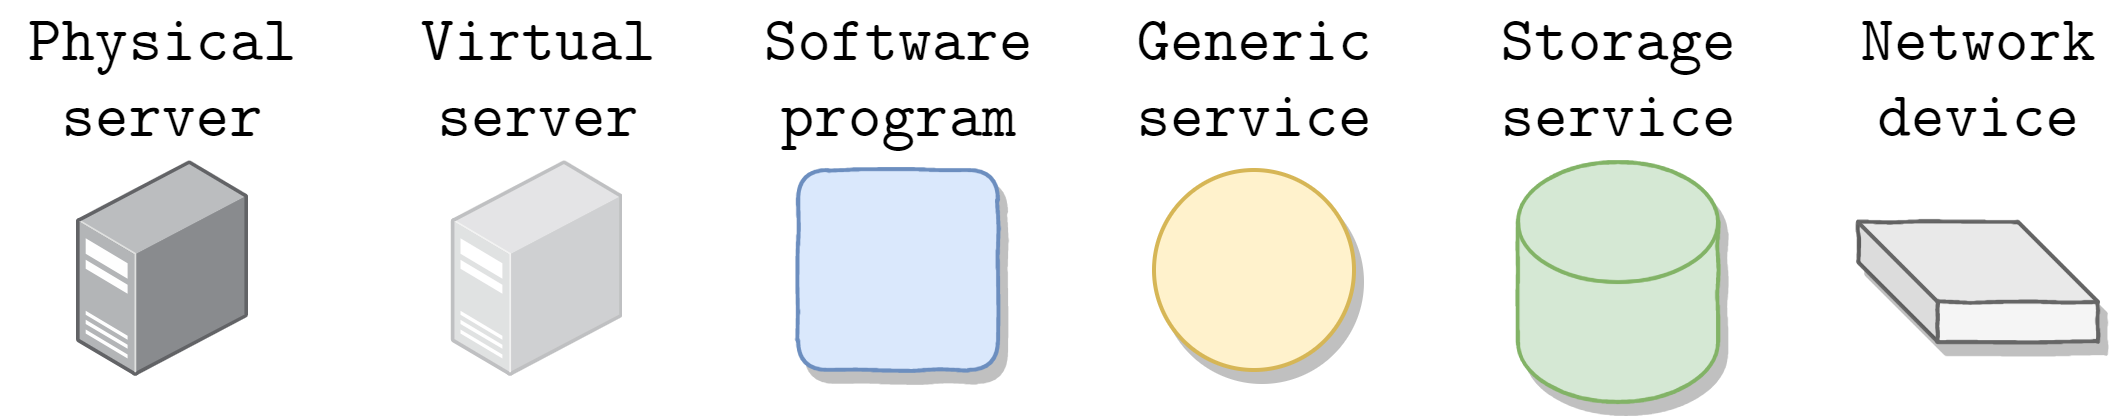
\includegraphics[width=8cm]{./Images/cap2/2.3.png}
    \label{fig:image2.3}
\end{figure}

Una risorsa ospitata nei confini dell'organizzazione a cui appartiene viene detta \textbf{on-premise}. Una risorsa on-premise non può essere cloud-based e viceversa, ma può accedere o interagire con una risorsa cloud-based. Esiste poi il \textit{Redudant deployment}, che permette di avere risorse sia on-premise che su cloud, aumentando l'affidabilità.
\subsection{Scaling}
Lo scaling rappresenta la capacità di una risorsa di poter gestire le richieste d'uso (che aumentano e diminuiscono), mantenendo la stessa architettura. Esistono due tipi di scaling.
\subsubsection{Horizontal scaling}
L'Horizontal scaling è quello tipico dei sistemi distribuiti, e consiste nell'allocare o rilasciare risorse di uno stesso tipo. Ad esempio, supponiamo di avere a disposizione un certo numero di server fisici e un numero di server virtuali che possono essere aumentati per offrire piu risorse di calcolo (scaling out) o diminuiti per ridurre gli sprechi quando non tutti vengono utilizzati (scaling in).
\begin{figure}[ht]
    \centering
    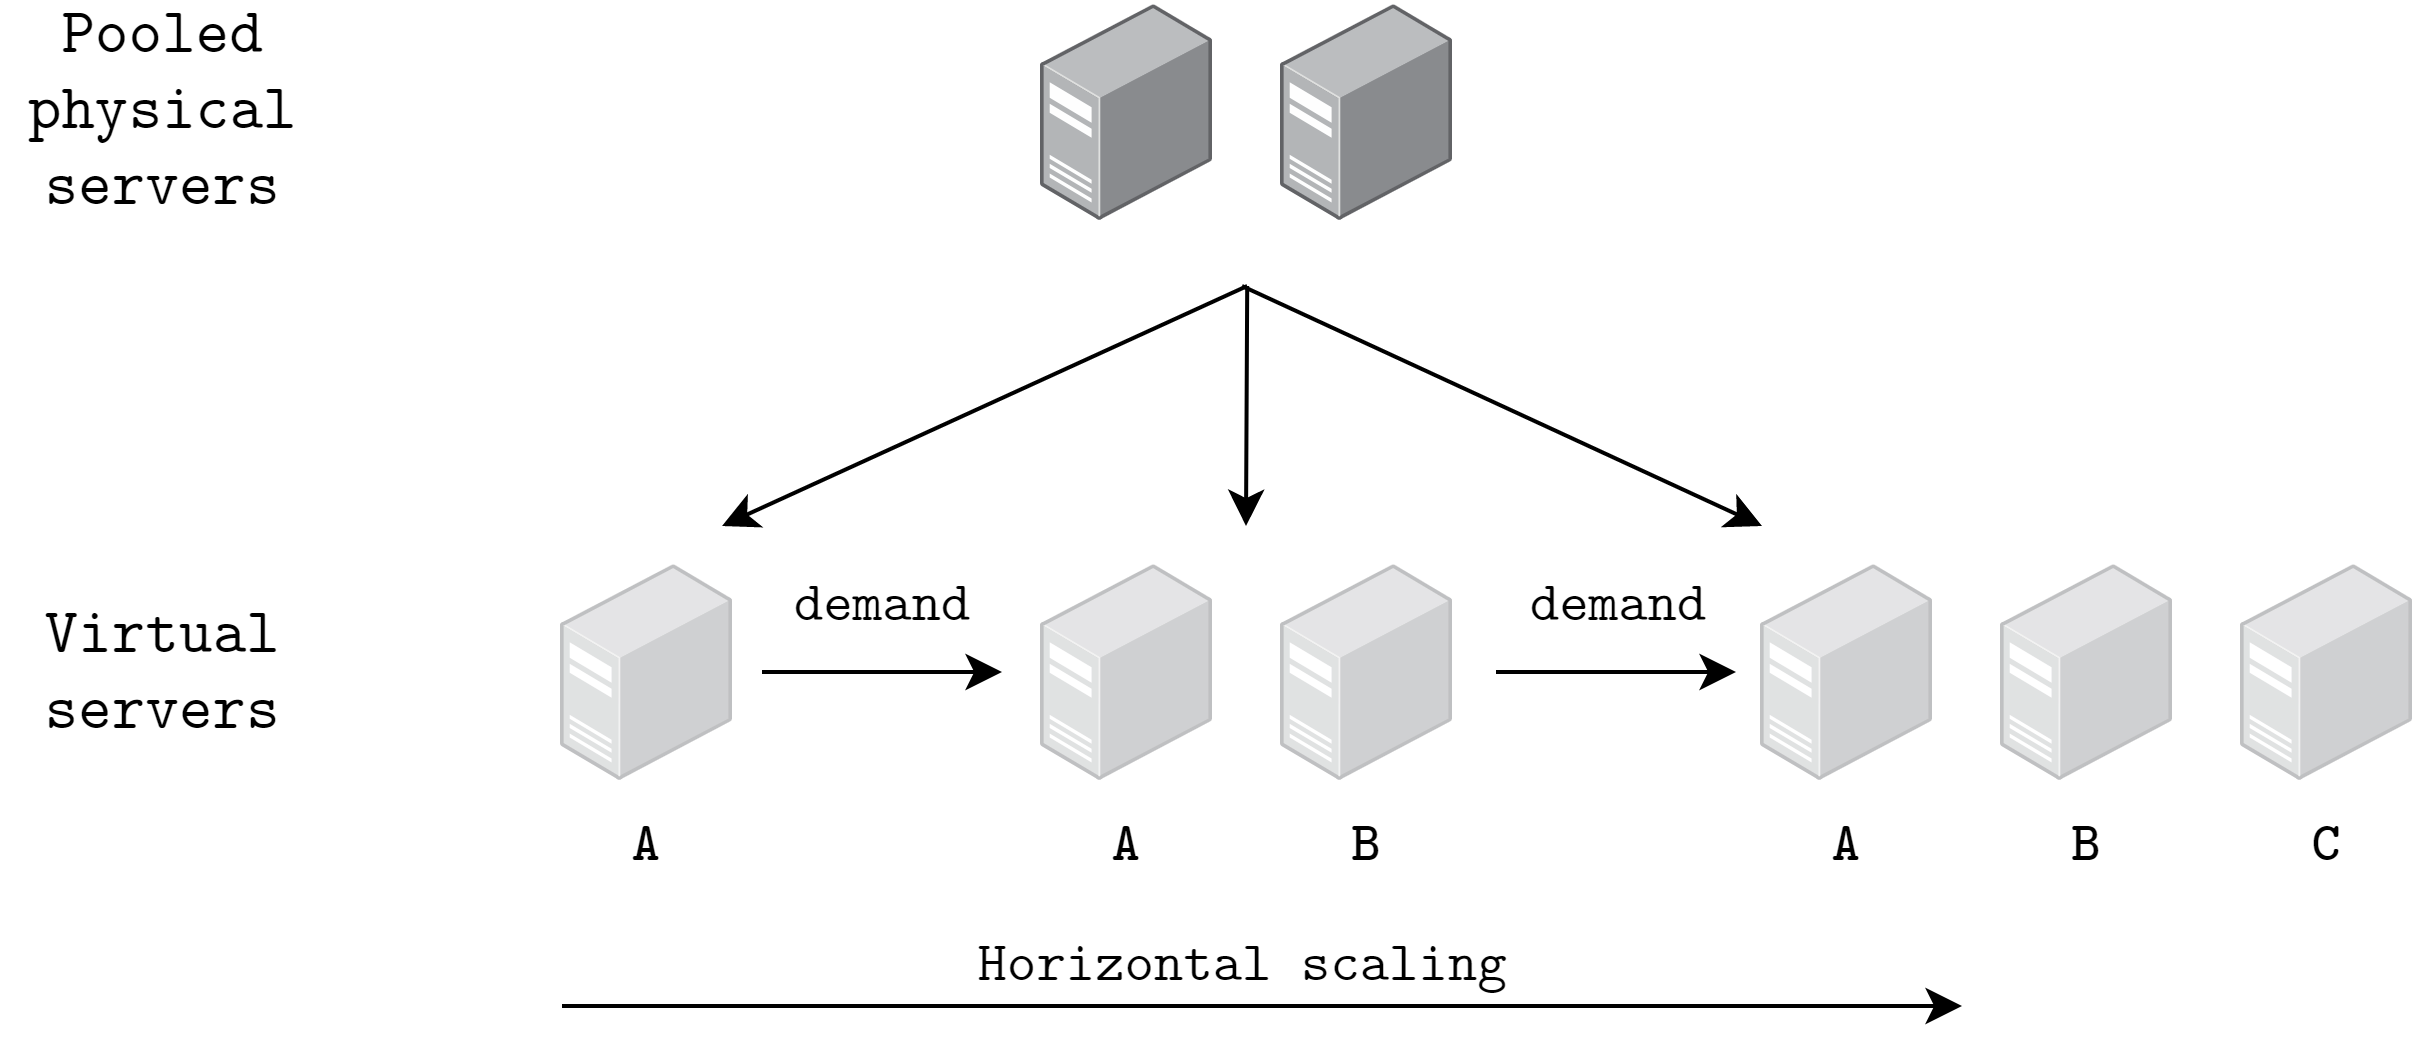
\includegraphics[width=9cm]{./Images/cap2/2.4.png}
    \label{fig:image2.4}
\end{figure}

\subsubsection{Vertical scaling}
Il vertical scaling permette di eseguire una risorsa con più o meno capacità, ad esempio come dare più CPU a una risorsa (scaling up), o meno storage ad un altra risorsa (scaling down). In breve, le risorse hardware utilizzate sono le stesse ma possono essere rese più o meno performanti a seconda della domanda. 
\vspace{5mm}

Il vertical scaling, a differenza di quello orizzontale, non è potenzialmente infinito, in quanto è limitato dalla capacità dell'hardware, tuttavia è estremamente veloce ed efficace. Inoltre l'horizontal scaling utilizza lo stesso hardware che è possibile trovare normalmente in commercio (se voglio costruire un cluster posso benissimo acquistare 100 computer e gestirmeli da solo); il vertical scaling utilizza invece hardware specializzato.
\subsection{Service Level Agreement}
Le condizioni di utilizzo di un \textbf{cloud service} sono spesso indicate in un accordo chiamato \textbf{Service Level Agreement} (SLA). Uno SLA è scritto in linguaggio naturale (quindi è leggibile da umani) e mette in relazione il cloud provider con il cloud consumer, stabilendo e garantendo la \textbf{Quality of Service} (QoS). È una specifica critica nel mondo del cloud computing, perché nella stragrande maggioranza dei casi le implementazioni delle architetture sono nascoste al cloud consumer\footnote{Un cloud consumer spesso è anche indicato come \textbf{Cloud Service Consumer},ruolo temporaneo che viene assunto quando usufruisce di un servizio cloud.}.
\section{Obiettivi e benefici}
Come in precedenza sono state affrontate le tecnologie che hanno permesso lo sviluppo e l'evoluzione del cloud computing, ora analizziamo quali sono gli obiettivi principali e i benefici che esso porta.
\subsection{Reduced Investments and Proportional Costs}
Il problema di acquistare hardware e software e i costi di manutenzione impattano in maniera forte su un centro di calcolo, quindi la possibilità di effettuare accessi on-demand pagando solo per ciò che si usa è uno degli obiettivi del cloud computing. La percezione di avere risorse infinite riduce il bisogno di ricorrere a planning e provisioning, e questo garantisce un beneficio all'azienda che affidandosi a servizi cloud riducendo i costi dell'hardware può concentrarsi sul suo obiettivo principale.
Inoltre c'è un livello di scelta molto granulare, che permette di evitare la necessità di \textit{upfront committments}. Inoltre l'infrastruttura delle macchine non è vincolata fisicamente, il che significa che è possibile spostarla con relativa facilità.
\subsection{Increased Scalability}
Grazie alla scalabilità il cloud può allocare dinamicamente risorse in modo molto veloce. Ad esempio, se so che il mio servizio viene utilizzato prevalentemente dalle 10 alle 22, posso organizzare le risorse per fare in modo che scalino in base al traffico che si genera sulla piattaforma, e posso impostare un limite per tutelarmi da eventuali spese non considerate. Le strategie di business driver utilizzate in questi casi sono \textit{lag strategy} e \textit{match strategy}.
\begin{figure}[ht]
    \centering
    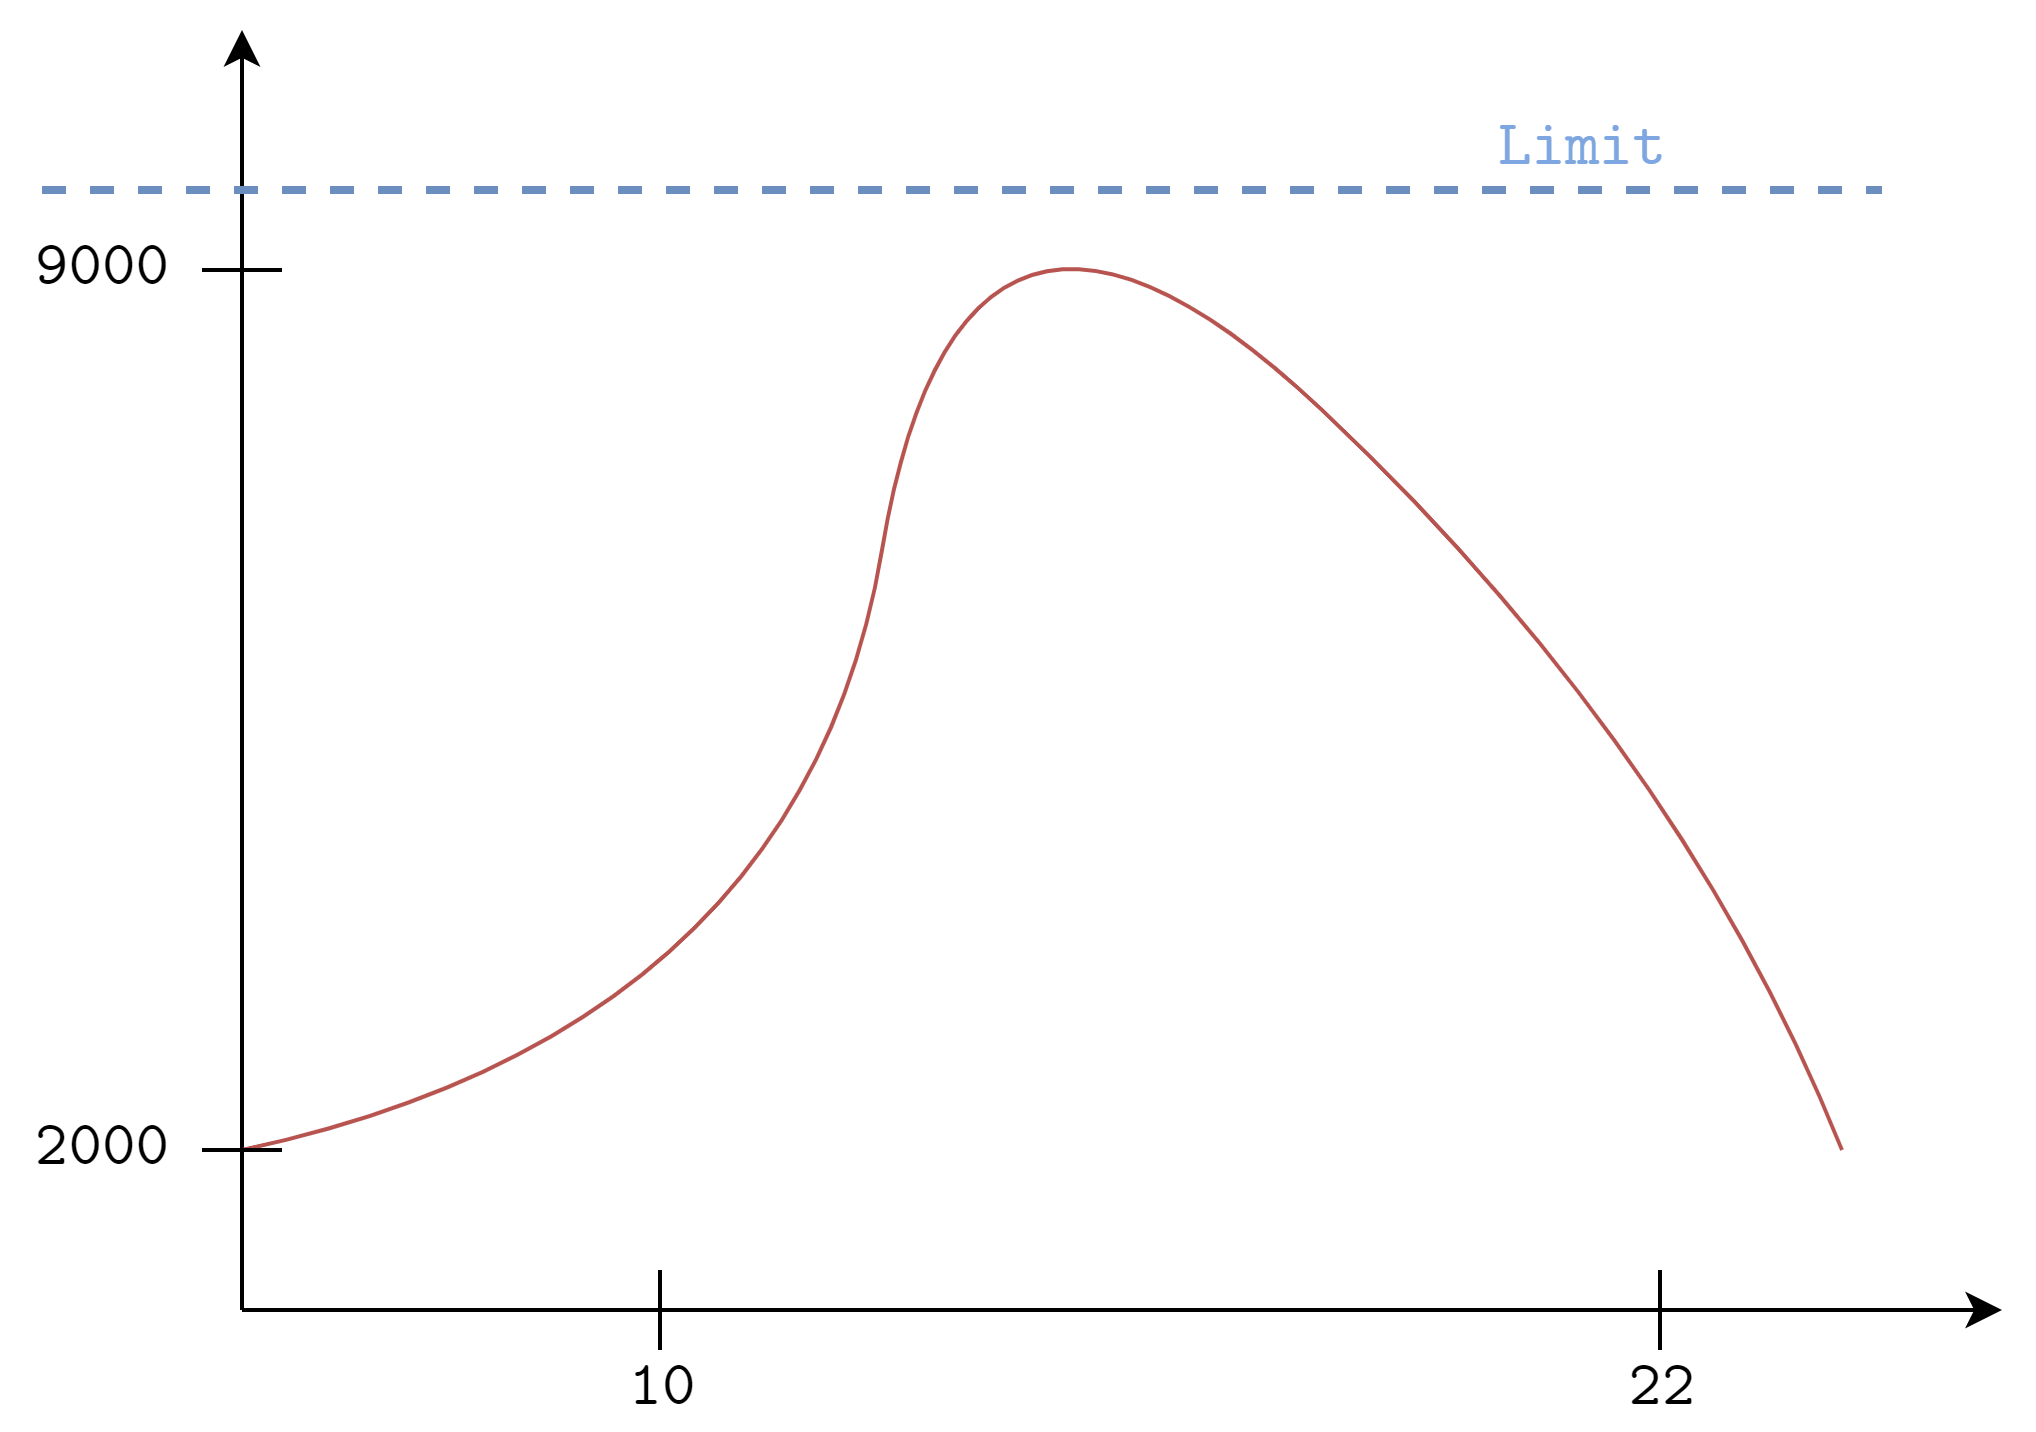
\includegraphics[width=7cm]{./Images/cap2/2.5.png}
    \label{fig:image2.5}
\end{figure}

\subsection{Increased Availability and Reliability}
La struttura modulare delle architetture cloud permettono di far fronte a diversi problemi che si verificano spesso, come tempi di downtime necessari, che possono essere annullati grazie alla disponibilità di più macchine che possono essere interscambiate per effettuare le stesse operazioni.
Le risorse IT che hanno maggiore affidabilità riescono anche ad evitare più facilmente le condizioni di fallimento.

\begin{mdframed}[backgroundcolor=gray!20,shadow=false]
\textbf{Summary of Key Points}
\begin{itemize}
    \item Gli ambienti cloud comprendono un'estesa infrastruttura che offre una serie di risorse IT che possono essere noleggiate utilizzando un modello \textit{pay-per-use}. Messi a confronto con ambienti equivalenti on-premise, hanno il potenziale per ridurre gli investimenti iniziali e i costi operazionali.
    \item L'abilità di un cloud di scalare le risorse permette alle organizzazioni di sostenere cambiamenti imprevedibili di utilizzo delle risorse senza far fronte a quei costi che dovrebbero essere sostenuti senza cloud.
    \item Utilizzando il cloud per aumentare la disponibilità di risorse a disposizione, le aziende possono aumentare la qualità del servizio offerto e ridurre o evitare del tutto potenziali perdite di utenti e di denaro.
\end{itemize}
\end{mdframed}

\section{Risks and Challenges}
Esistono principalmente quattro principali categorie di rischio:
\begin{itemize}
    \item \textbf{Increased security vulnerabilities}: con il cloud si ha un'espansione dei \textit{trust boundaries}, ovvero è come se l'azienda diventasse più grande. Il cloud provider ha accesso ai nostri dati, e nonostante siano implementati metodi di crittografia end-to-end per la comunicazione, questi boundaries estesi possono essere vittima di interventi maliziosi. Di seguito è illustrato uno scenario dove due aziende che si affidano allo stesso cloud provider devono convivere con una situazione che viene chiamata di \textbf{boundaries overlapping}: i dati presenti nel cloud possono costituire un rischio per le aziende.
    
    \begin{figure}[ht]
    \centering
    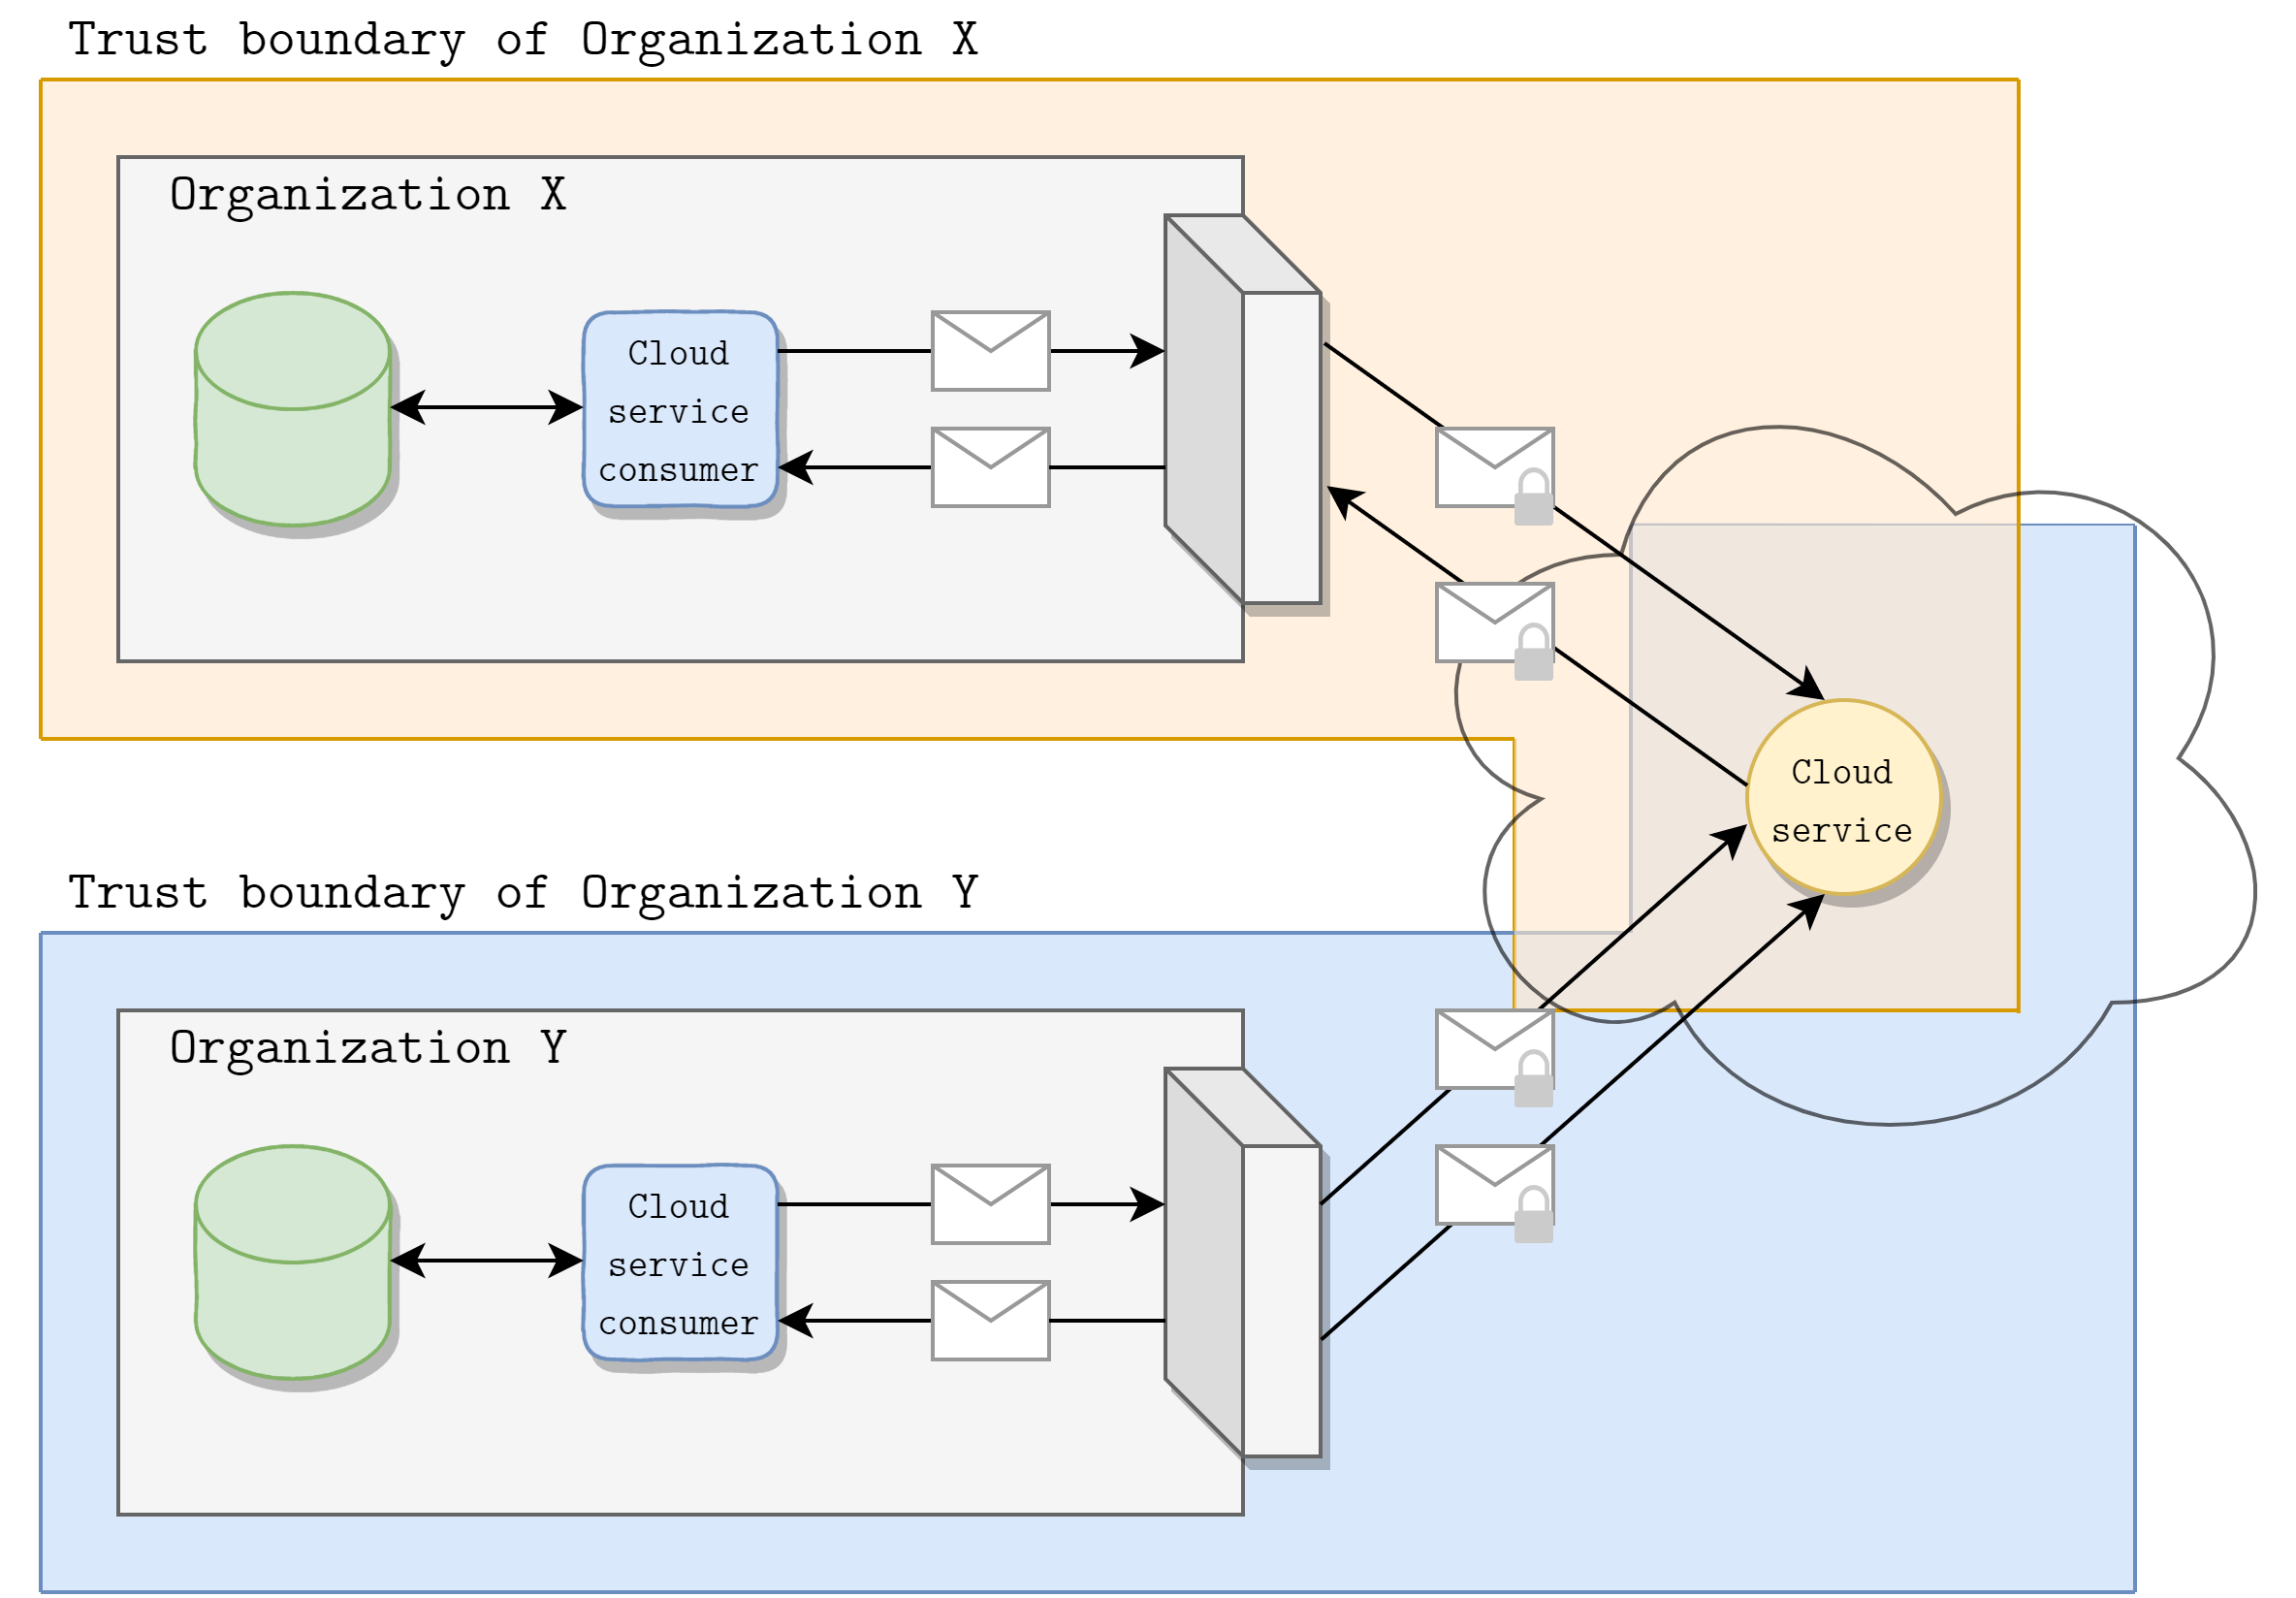
\includegraphics[width=9cm]{./Images/cap2/2.6.png}
    \label{fig:image2.6}
\end{figure}
    
    \item \textbf{Reduced operational governance control}: significa che i cloud consumer devono considerare rischi derivanti dalla lontananza delle regioni in cui si trovano le infrastrutture che ospitano le loro risorse sul cloud. Ad esempio, queste distanze potrebbero richiedere ulteriori step di connessione e introdurre vincoli di larghezza di banda, che causano problemi di connessione e l'impossibilità di accedere alle risorse.
    \item \textbf{Limited portability between cloud providers}: di norma le tecniche utilizzate per la costruzione delle infrastrutture cloud sono proprietarie a causa della mancanza di standard nell'industria del cloud computing, per cui potrebbe risultare difficile o in certi casi impossibile spostare su un altro cloud l'infrastruttura hostata da un certo cloud provider. È chiaro che ci sono principalmente problemi di portabilità e di migrazione, ad esempio un certo cloud su cui metto a disposizione le mie risorse potrebbe fornire crittografia e firma digitale come sicurezza mentre un altro solo crittografia standard: in questo caso mi risulterebbe particolarmente complicato riorganizzare l'architettura per effettuare la migrazione.
    \item \textbf{Multi-regional compliance and legal issues}: i data center vengono costruiti di norma in posti quasi isolati e in regioni che offrono elettricità a buon prezzo. Il problema sta nel fatto che i dati presenti in quel cloud sono sottoposti alle leggi vigenti in quella regione, e nessuno mi garantisce che siano le stesse che vigono nel paese in cui mi trovo. I dati devono sempre essere tutelati, ma spesso accade che i cloud consumer non sanno neanche in che regioni stanno i loro dati. 
    Alcuni esempi: a seguito della Brexit la società ServiceNow ha spostato molte delle sue infrastrutture dal Regno Unito in Olanda, per garantire la tutela delle normative europee. Un cloud consumer europeo dovrebbe fare attenzione ai suoi dati se sono hostati negli USA, in quanto secondo il Patriot Act qualsiasi organizzazione governativa può accedere ai dati presenti nel territorio statunitense.
\end{itemize}

\begin{mdframed}[backgroundcolor=gray!20,shadow=false]
\textbf{Summary of Key Points}
\begin{itemize}
    \item Gli ambienti cloud possono introdurre diverse sfide di sicurezza, alcune delle quali portano al fenomeno del \textit{boundary overlapping}, nel quale un cloud provider condivide le stesse risorse con più cloud consumer.
    \item Le scelte operazionali di un cloud consumer possono essere limitate dagli ambienti ospitati dal cloud a causa del controllo esercitato da un cloud provider sulle sue piattaforme.
    \item La portabilità delle risorse cloud-based può essere compromessa dalle dipendenze di caratteristiche proprietarie imposte da un cloud provider.
    \item La posizione geografica dei dati e delle risorse potrebbero trovarsi fuori dal controllo di un cloud consumer nel caso fossero ospitate da un cloud provider di terze parti. Questo potrebbe causare diversi problemi o incongruenze a livello legale, perché la maggior parte delle volte le leggi indicano come responsabile il cloud consumer e non il cloud provider.
\end{itemize}
\end{mdframed}

\section{Learning Check}
Alla fine di ogni capitolo verranno elencate delle domande che potrebbero essere poste all'esame.
\begin{enumerate}
    \item Descrivi la diffusione del cloud computing partendo da una combinazione di business drivers e innovazioni tecnologiche e descrivi l'evoluzione delle definizioni associate al cloud computing.
    \item Descrivi le responsabilità e le sfide del capacity planning per le organizzazione IT e spiega il problema dei costi operazionali per le aziende che presentano requisiti di utilizzo variabili e/o imprevedibili.
    \item Spiega il bisogno di agilità organizzativa per un'azienda IT di rispondere a cambiamenti del business.
    \item Spiega il concetto di grid computing e la definizione del modello \textit{pay-as-you-go}.
    \item Spiega la natura demand-driven e le tecnologie delle architetture di back-end che sono comunemente utilizzate nelle applicazioni web.
    \item Spiega la causa della diffusione del cloud computing come un campo distinto di competenza risultante dai business drivers e dalle innovazioni tecnologiche.
    \item Descrivi il termine "servizio" nel contesto del cloud computing e spiega cosa costituisce una risorsa IT.
    \item Descrivi l'horizontal scaling e i due tipi di horizontal scaling, il vertical scaling e i due tipi di vertical scaling.
    \item Spiega perché la virtualizzazione è una tecnologia chiave degli ambienti del cloud computing, e i benefici di un ambiente virtualizzato.
    \item Spiega da cosa è formato un cloud e la differenza tra una risorsa on-premise e una risorsa cloud-based.
    \item Spiega cosa vuol dire "servizio" da una prospettiva IT e cosa costituisce un servizio cloud (cloud service).
    \item Spiega cos'è un \textit{service agent} e perché è comunemente usato nel cloud.
    \item Descrivi i benefici degli investimenti ridotti e dei costi propozionali e spiega la relazione di questi benefici con il modello \textit{pay-per-use}, e come il beneficio dei costi di noleggio di risorse IT cloud-based differisce da quello delle risorse on-premise.
    \item Descrivi il beneficio della \textit{Increased Scalability} e spiega come questo beneficio può essere in relazione con la reattività di un'organizzazione.
    \item Descrivi il beneficio della \textit{Increased Availability and Reliability} e spiega come questo beneficio può essere in relazione con il supportare situazioni di fallimento, e come è fornito in maniera trasparente ai cloud consumer.
    \item Descrivi la sfida che caratterizza le \textit{Increased Security Vulnerabilities} e spiega come questa sfida può essere messa in relazione all'espansione e all'overlapping dei trust boundariese come può essere in relazione con i problemi di compatibilità e di sicurezza tra cloud provider e cloud consumer. 
    \item Descrivi il rischio scaturito dal \textit{Reduced Operational Governance Control} e spiega come questo rischio sorge negli ambienti cloud e come è in relazione con l'utilizzo dei SLA da parte dei cloud consumer. Spiega poi anche come questo rischio può portare a problemi nel caso di cloud provider irresponsabili.
    \item Descrivi la sfida della portabilità limitata tra cloud provider e spiega perché i cloud provider impongono caratteristiche proprietarie nei loro cloud, indicando il ruolo degli standard industriali in relazione con questa sfida.
    \item Descrivi i rischi causati dal fenomeno del \textit{Multi-Regional Compliance} e spiega come problemi di natura legale possono sorgere a causa della posizione geografica dei dati di un cloud consumer.
\end{enumerate} 

